\documentclass{article}

% if you need to pass options to natbib, use, e.g.:
% \PassOptionsToPackage{numbers, compress}{natbib}
% before loading nips_2018

% ready for submission
\usepackage[final]{nips_2018}

% to compile a preprint version, e.g., for submission to arXiv, add
% add the [preprint] option:
% \usepackage[preprint]{nips_2018}

% to compile a camera-ready version, add the [final] option, e.g.:
% \usepackage[final]{nips_2018}

% to avoid loading the natbib package, add option nonatbib:
% \usepackage[nonatbib]{nips_2018}

\usepackage[utf8]{inputenc} % allow utf-8 input
\usepackage[T1]{fontenc}    % use 8-bit T1 fonts
\usepackage{hyperref}       % hyperlinks
\usepackage{url}            % simple URL typesetting
\usepackage{booktabs}       % professional-quality tables
\usepackage{amsfonts}       % blackboard math symbols
\usepackage{nicefrac}       % compact symbols for 1/2, etc.
\usepackage{microtype}      % microtypography
\usepackage{graphicx}
\usepackage{hyperref}
\hypersetup{
    colorlinks=true,
    linkcolor=blue,
    filecolor=magenta,      
    urlcolor=cyan,
}
\usepackage{subcaption}

\title{Project Report}

% The \author macro works with any number of authors. There are two
% commands used to separate the names and addresses of multiple
% authors: \And and \AND.
%
% Using \And between authors leaves it to LaTeX to determine where to
% break the lines. Using \AND forces a line break at that point. So,
% if LaTeX puts 3 of 4 authors names on the first line, and the last
% on the second line, try using \AND instead of \And before the third
% author name.

\author{M.P.Ross}

\begin{document}

\maketitle

\begin{abstract}
Multimessenger astronomy using gravitational waves require low latency event classification and localization. Previous studies have studied searching for binary coalescence waveforms using machine learning with strain time series as the input and found that Deep Neural Networks were required to get accurate results. I'm studying applying machine learning to searching for both supernovae and binary coalescence events using the Fourier transform as the inputs.
\end{abstract}

\section{Introduction}
Gravitational waves (GW) are ripples in space time which are emitted by rapidly changing mass quadrupole moments. The only sources that are known to emit these in measurable quantities are cataclysmic astrophysical events including binary neutron star mergers, binary black hole coalescence, and core collapse supernovae. The LIGO/Virgo collaboration has measured GW from ten binary black hole coalescence and one binary neutron star merger using 4 km long L-shaped interferometric observatories, located in Hanford, WA, Livingston, LA, and Pisa, Italy [5]. These observatories work by measuring the differential strain along the two arms of the observatory. To triangulate the source's location on the sky we need two or more distant detectors operating simultaneously.

For most events types, GW are emitted slightly before any light; the delay being around a few seconds. Subsequently, one of the goals of our observations is to alert optical telescopes to point towards the source before the light arrives to allow for so called multimessenger astronomy. To achieve this, we need to analyze the strain channel with the smallest latency possible to allow the telescopes to have enough time to point towards the source. Additionally, some of these events are buried within instrumental noise so complex algorithms are needed to extract them. Currently, the analysis consists of matched filtering or looking for any coherent burst in a set of detectors. Both of these methods are computationally intensive and increase the time between arrival and detection. Machine learning has gained attention lately as a possible alternative to achieve low latency detections. Previous studies have focused on compact binary coalescence (CBC) signals as they are the most probable event types (and due to the fact that we've already measured a collection of them) [2, 3]. Additionally, they used the raw time series as the inputs into their neural networks. 

Here, I apply machine learning techniques to detect both CBC and supernova events using the Fourier transform of the time series as the input to test the hypothesis that this preprocessing will decrease the complexity needed to make accurate detections. Other authors [2, 3, 4] have attempted to use ML for both detection and estimating the properties of the emitting system but here I am restricting the scope to only detection. The goal of the algorithm is to place each event into either containing a GW event or not.

\section{Data sets}
\subsection{Supernova}
Supernova are cataclysmic outburst that occur in the process of the a main sequence star collapsing at the end our their life to become either a neutron star or a black hole. During these events extreme amounts of matter are thrown out in in a chaotic fashion which is theorized to lead to emission of gravitational waves.

Due to the lack of true measurements of gravitational waves from core collapse supernovae, to train an algorithm we must rely on synthetic data sets to train our algorithms. To make the data as realistic as possible, a set of real strain data was taken from the observatories which does not contain any known GW events (this series is referenced later as noise) and theoretical supernovae waveforms were injected. The noise data was obtained from the LIGO Open Science Center (\href{https://www.gw-openscience.org/about/}{https://www.gw-openscience.org/about/}) and the waveforms were calculated by the GW theory group at the Max Planck Institute (\href{https://www.mpa-garching.mpg.de/177514/Gravitational-Waveform-Catalog}{https://www.mpa-garching.mpg.de/177514/Gravitational-Waveform-Catalog}).

In order to study the characteristics of the decreased SNR, I generated a collection of sets corresponding to event distances between 1 kpc to 100 kpc. Due to the quadrople nature of GW, the amplitude decreases as $1/r$ which allowed for easy manipulation using a simple gain factor on the injected signal. True SNR is more difficult to obtain since each waveform corresponds to a different mechanism with a unique amount of emitted GW. Due to this fact, I opted to let distance be a rough proxy for SNR.

To cover the entire range of waveform types and many noise conditions, I generated a set of 276 one second long time series half of which had a waveform injected and the other half only containing noise. The noise for each data series was drawn with a random beginning time from the same 1000 second noise time series. For the data sets that contain an injection, a waveform was drawn randomly from a set of 138 and placed at a random time within the one second long noise time series.  Below is an example of a time series with and without the injected signal and it's corresponding power spectral density (PSD).

\begin{figure*}[h!]
    \centering
    \begin{subfigure}[t]{0.5\textwidth}
        \centering
        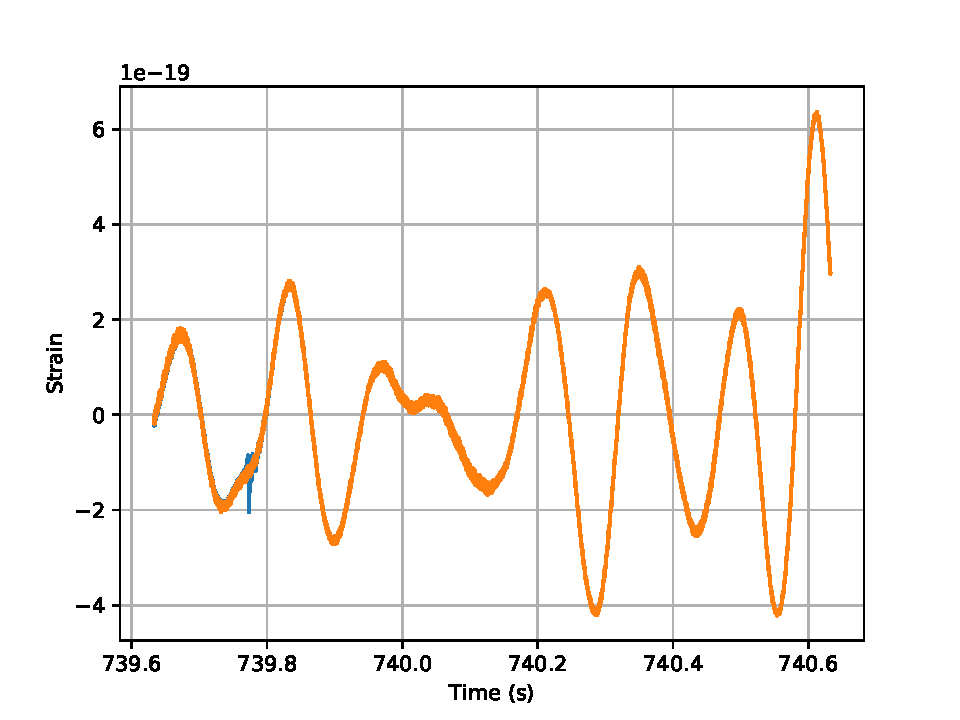
\includegraphics[height=2in]{TimeSeries.pdf}
    \end{subfigure}%
    ~ 
    \begin{subfigure}[t]{0.5\textwidth}
        \centering
        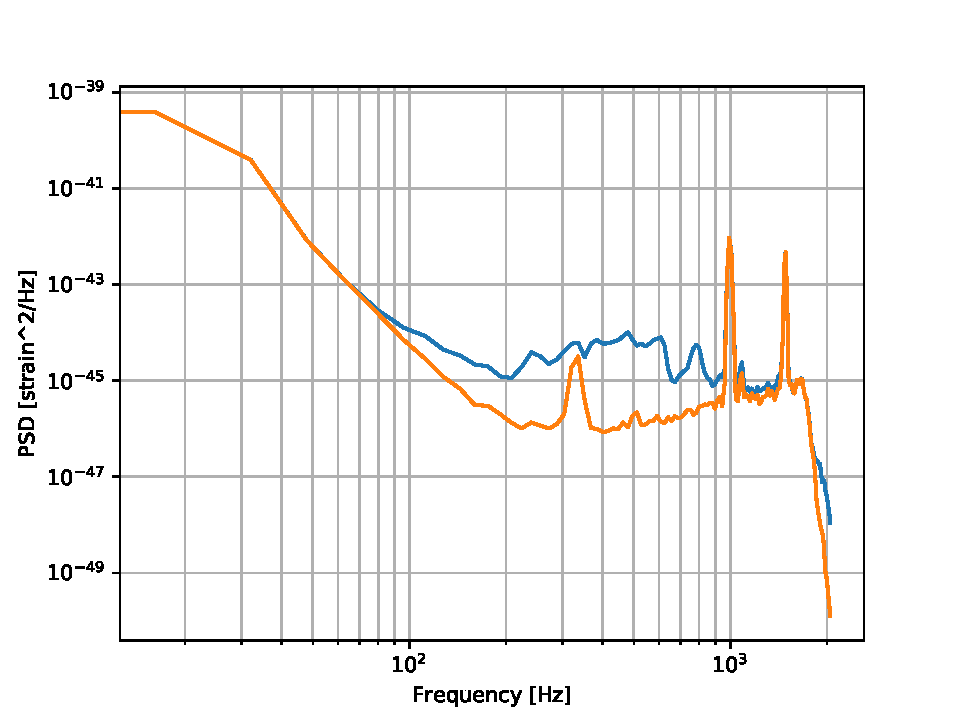
\includegraphics[height=2in]{PSD.pdf}
    \end{subfigure}
    \caption{Time series (left) and power spectral density (right) of a selected synthetic data set corresponding to a supernova within 1 kpc with orange being the noise and blue showing the injected waveform. }
\end{figure*}

While generating the supernova waveforms, I quickly found that if I attempted to increase the size of that data set using the same bank of 138 waveforms, I achieved artificially good performance due to the fact that the testing and training datasets quickly became mirrors of each other. This is a fundamental limitation of using ML to hunt for Supernova signal because there's is only a small number of Supernova waveforms that have been generated using costly numerical simulations. CBC searches do not suffer from this limitation due to readily available libraries that use analytical approximations to generate waveforms on demand.

\subsection{CBC}

Compact binary coalescence is the process of two massive objects, either black holes or neutron stars, that orbit a common center of mass, undergoing orbital decay due to the emission gravitational waves and eventually merging. These events emit extreme amounts of energy in the form of GW which make them the easiest events to measure and study. The amplitude and frequency content of the GW emitted by these event are functions of the masses of the objects, higher mass gives larger amplitude but lower frequency. We have measured a total of eleven, ten binary black hole mergers and one neutron star merger, which restrict our ability to use true measurements to train algorithms. 

Subsequently, I generated another synthetic data set half containing injected CBC events and half containing only noise in a similar fashion as the Supernova data set. To cover the parameter space which overlaps and exceeds the current list of observations, I injected waveforms drawn from a bank consisting of 1000 waveforms generated using the pyCBC package (\href{https://pycbc.org/}{https://pycbc.org/}) ranging from 10 solar masses to 100 solar masses. 

\section{Training}

To test whether multilayer convolutional neural networks, like those created in [2, 3, 4], are necessary to get good detection accuracy, I wanted to test a selection of simple methods with a more complex one. I selected a set of four algorithm implemented in sklearn: logistic regression, nearest neighbor, SVM, and a simple prebuilt neural network. Additionally, I developed a convolutional neural network (CNN) consisting of a single convolution layer and a single linear layer. My hopes are that this will do better than the sklearn methods yet be simple enough to have computational speed up verses a multilayer design. All of these methods were tuned for each separately for the CBC and Supernova data sets and trained on half of the given data while the other half was used for testing.

\begin{figure*}[h!]
    \centering
    \begin{subfigure}[t]{0.5\textwidth}
        \centering
        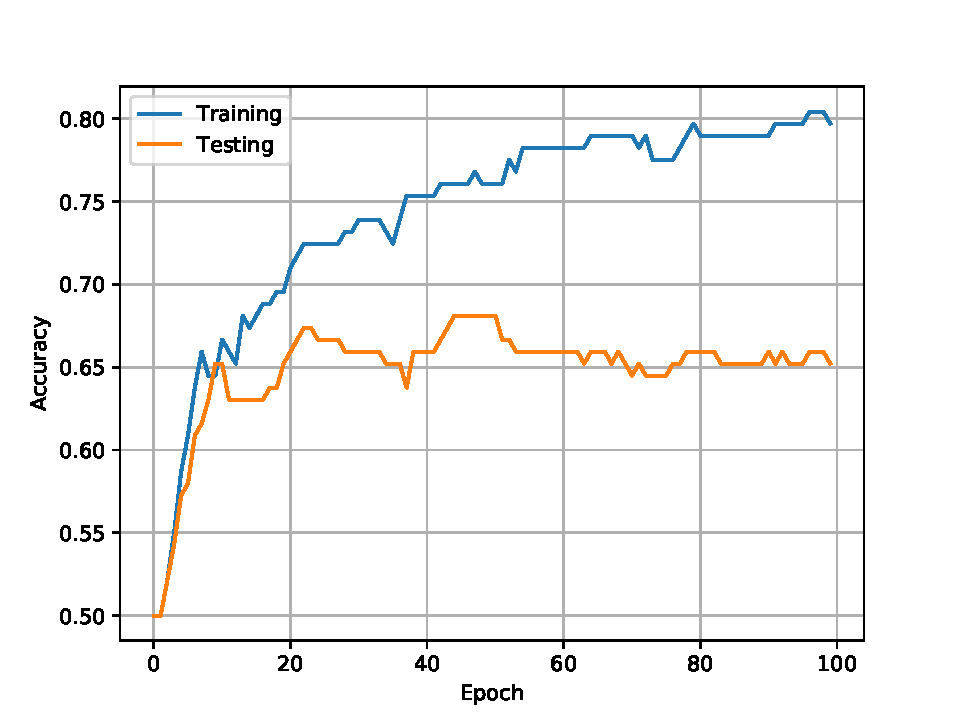
\includegraphics[height=2in]{NNTrainingSN.pdf}
    \end{subfigure}%
    ~ 
    \begin{subfigure}[t]{0.5\textwidth}
        \centering
        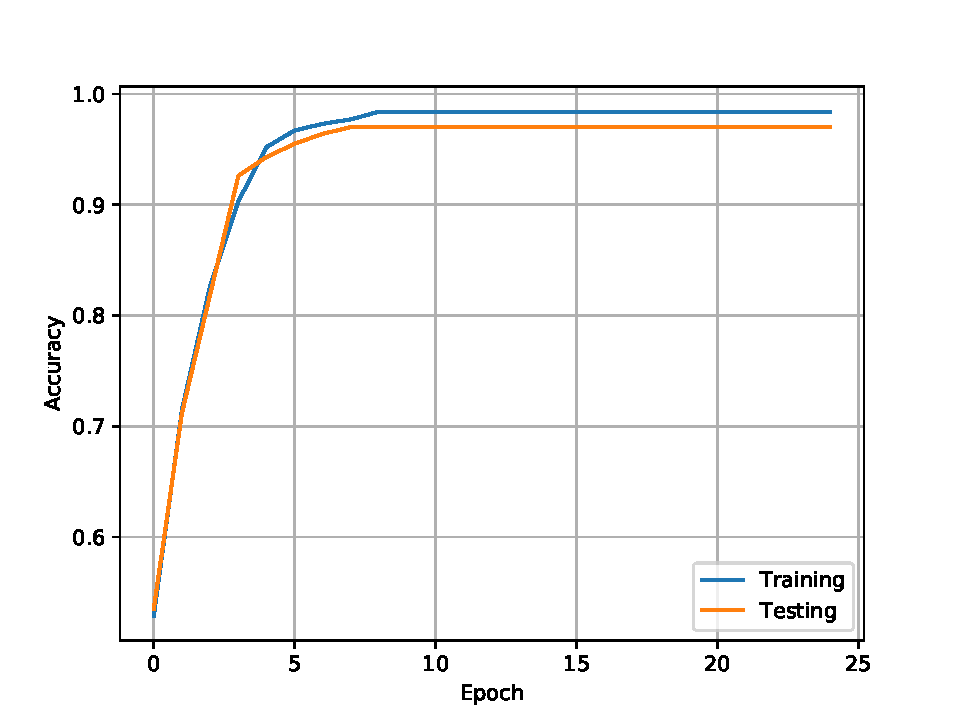
\includegraphics[height=2in]{NNTrainingCBC.pdf}
    \end{subfigure}
    \caption{Training and testing error of the CNN for the Supernova (left) and CBC (right) data sets vs. training epoch.}
\end{figure*}

\section{Results}

To accurately compare the collection of algorithms, each was trained and tuned at a given distance (2 Mpc for CBC, 50 kpc for Supernova) and then applied to the others, shown in Figure 3. This additionally, allows for a more accurate estimation of the true error due to the fact that these other data sets were not used during the hyper parameter tuning and are thus more independent.

\begin{figure*}[h!]
    \centering
    \begin{subfigure}[t]{0.5\textwidth}
        \centering
        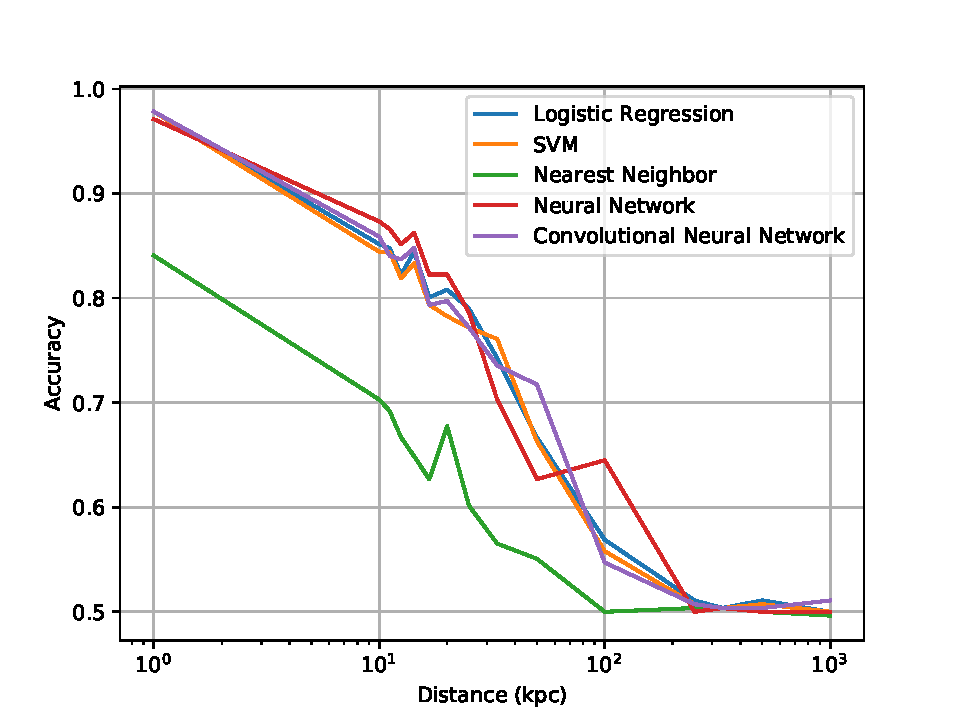
\includegraphics[height=2in]{AccuracyDistanceSN.pdf}
    \end{subfigure}%
    ~ 
    \begin{subfigure}[t]{0.5\textwidth}
        \centering
        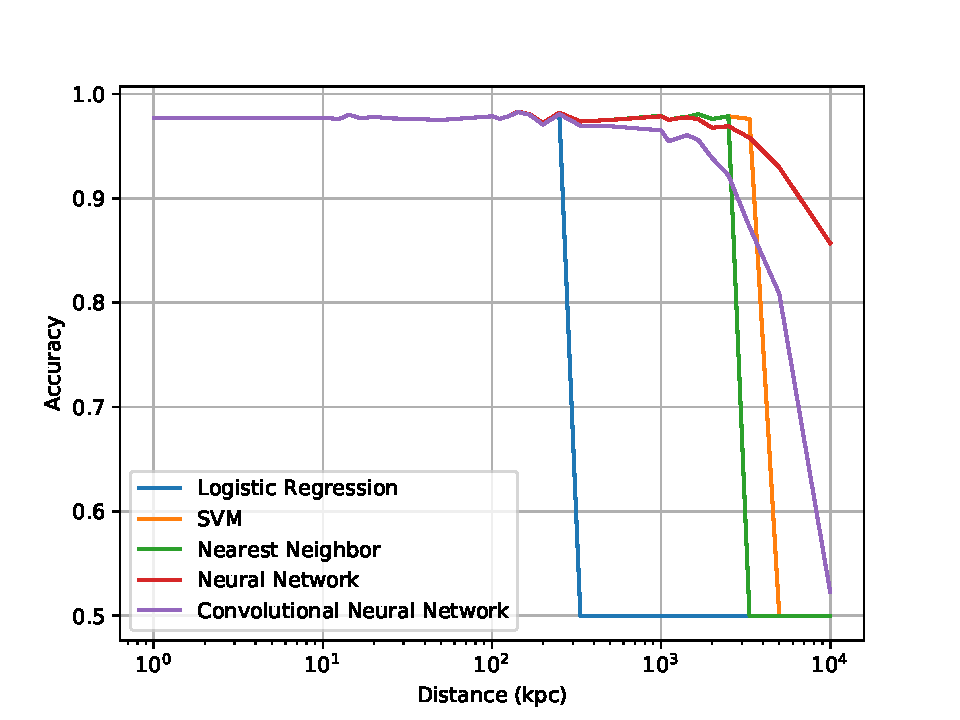
\includegraphics[height=2in]{AccuracyDistanceCBC.pdf}
    \end{subfigure}
    \caption{Accuracy of the collection of methods for the Supernova (left) and CBC (right) data sets with at a given distance.}
\end{figure*}

With the CNN tuned for the CBC data set, I have the unique ability to test the performance on the eleven measured GW events [5]. To do this I evaluated the CNN on 4096 second long data sets each contain one event. If the algorithm was perfectly accurate one would expect to find only one event per data set.

\begin{tabular}{ c | c | c | c | c | c  }
  GW150914 & GW151012 & GW151226 & GW170104 & GW170608 & GW170729\\
  \hline
  \hline
 1 & 0 & 0 & 0 & 2 & 0\\
 \end{tabular}
 
 \begin{tabular}{ c | c | c | c | c  }

GW170809 & GW170814 & GW170817 & GW170818 & GW170823 \\
   \hline
 \hline
   0 & 0 & 0 & 0 & 0 \\  
\end{tabular}


\section{Conclusion}

Unfortunately, the simple CNN that I developed does not perform any better than most of the prebuilt methods. Although further hyperparameter tuning may be able to obtain further accuracy, it is likely limited by the preprocessing. The good performance of the simple methods makes sense as the events are clearly separable from the noise in frequency space and the decrease in the accuracy with distance probably traces close to the cumulative SNR of the events. 

For the true events, it is not very surprising that the CNN found more events than were present since the preprocessing decreases the ability to tell what events are true and what are just instrumental transients. It is well known that our observatories have short duration, high amplitude transients or ``glitches'' caused by environmental or instrumental effects. Additionally, the increased ability to detect CBC vs Supernova can be attributed to the fact that CBC events are longer in duration which increases the signal in the Fourier domain.

All of the evidence suggests that the complex time domain based CNN that were developed by other authors are the best path forward. Shifting to the Fourier domain increases the computation efficiency with the cost of muddling the nature of the event.  However, all current ML applications to gravitational wave detection have been solely based on synthetic data so it is difficult to truly compare methods. 

With the upcoming observing run slated to begin next year, it is expected that the number of detections will increase dramatically. Past observing runs have detection rates of roughly one event per month while the next observing run will expect roughly one every few days; this is expected to increase in future observing runs due to increased sensitivity. With growing cumulative number of events and higher detection rate, machine learning can reasonably be expected to play a larger role in future gravitational wave observations.

\section*{References}
\medskip

\small

[1] Gossan, S.E., Sutton, P., Sutver, A., Zanolin, M., Gill, K., \ \& Ott, C.D\ (2016) Observing gravitational waves from core-collapse supernovae in the advanced detector era. {\it Phys. Rev. D} {\bf 93}, 042002

[2] George, D., \ \& Huerta, E.A\ (2018) 
Deep Learning for real-time gravitational wave detection and parameter estimation: Results with Advanced LIGO data. {\it Physics Letters B} {\bf 778}

[3] George, D., \ \& Huerta, E.A\ (2018) Deep neural networks to enable real-time multimessenger astrophysics. {\it Phys. Rev. D} {\bf 97}, 044039

[4] Gabbard, H., Williams, M, Hayes, F., \ \&  Messenger, C.\ (2018) Matching Matched Filtering with Deep Networks for Gravitational-Wave Astronomy. {\it
Phys. Rev. Lett.} {\bf 120}, 141103

[5] The LIGO Scientific Collaboration \ \& the Virgo Collaboration. (2018) GWTC-1: A Gravitational-Wave Transient Catalog of Compact Binary Mergers Observed by LIGO and Virgo during the First and Second Observing Runs. https://arxiv.org/abs/1811.12907

 

\end{document}